O \textit{Algoritmo Genético} é uma família de modelos computacionais inspirados pelo evolucionismo. Esses algoritmos são utilizados para encontrar soluções aproximadas de problemas de otimização. 

Para ser construído, esse algoritmo necessita de uma \textbf{função-objetivo}, que é a expressão matemática que será minimizada. A grande vantagem desse algoritmo é que não é necessário conhecer inteiramente a função, como as suas derivadas, por exemplo. O único conhecimento necessário é saber o valor da função para cada indivíduo.

O \textbf{indivíduo} é outro componente necessário para realizar o algoritmo. O indivíduo representa um dos valores no espaço de busca, ou seja, é uma das opções para o mínimo da função-objetivo ser alcançado. O conjunto de todos esses indivíduos representa a \textbf{população}, que é o grupo total de opções possíveis para a minimização \cite{lindenalgoritmos}.

O algoritmo construído pode ser dividido em etapas, que foram divididas de acordo com as gerações de populações. A figura \ref{fig:genetico_tikz} ilustra o processo do algoritmo genético feito neste trabalho com todas as etapas do processo de construção do algoritmo \cite{whitleyGAtutorial}.
\begin{figure}[h]
	\begin{center}
		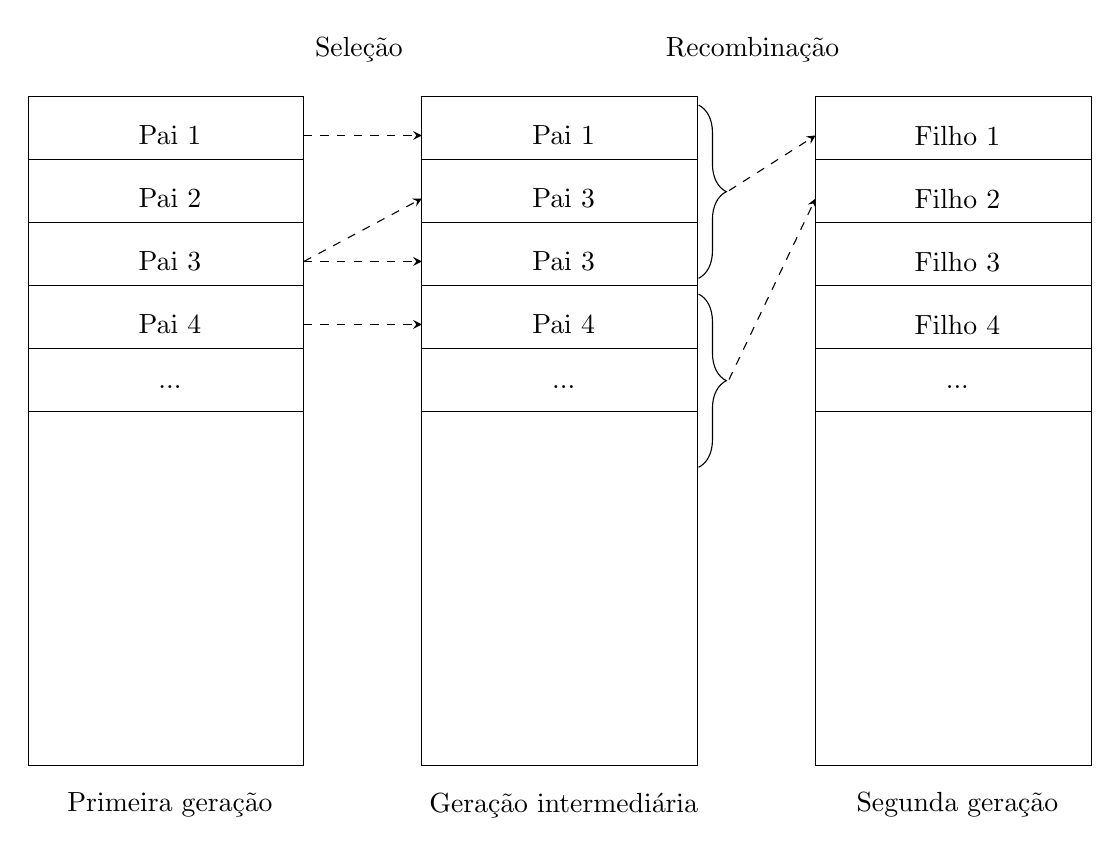
\begin{tikzpicture}
		
		
		\draw  (-5.0,4.0) rectangle (-1.5,-4.5);
		\draw  (0.0,4.0) rectangle (3.5,-4.5);
		\draw  (5.0,4.0) rectangle (8.5,-4.5);
		
		\draw [] (-5,3.2) -- (-1.5,3.2);
		\draw [] (-5,2.4) -- (-1.5,2.4);
		\draw [] (-5,1.6) -- (-1.5,1.6);
		\draw [] (-5,0.8) -- (-1.5,0.8);
		\draw [] (-5,0) -- (-1.5,0);
		
		\node at (-3.2,3.5) {Pai 1};
		\node at (-3.2,2.7) {Pai 2};
		\node at (-3.2,1.9) {Pai 3};
		\node at (-3.2,1.1) {Pai 4};
		\node at (-3.2,0.3) {...};
		
		\draw [dashed, -stealth] (-1.5,3.5) -- (0,3.5);
		\draw [dashed, -stealth] (-1.5,1.9) -- (0,2.7);
		\draw [dashed, -stealth] (-1.5,1.9) -- (0,1.9);
		\draw [dashed, -stealth] (-1.5,1.1) -- (0,1.1);
		
		\draw [] (0,3.2) -- (3.5,3.2);
		\draw [] (0,2.4) -- (3.5,2.4);
		\draw [] (0,1.6) -- (3.5,1.6);
		\draw [] (0,0.8) -- (3.5,0.8);
		\draw [] (0,0) -- (3.5,0);
		
		\node at (1.8,3.5) {Pai 1};
		\node at (1.8,2.7) {Pai 3};
		\node at (1.8,1.9) {Pai 3};
		\node at (1.8,1.1) {Pai 4};
		\node at (1.8,0.3) {...};
		
		\draw [] (5,3.2) -- (8.5,3.2);
		\draw [] (5,2.4) -- (8.5,2.4);
		\draw [] (5,1.6) -- (8.5,1.6);
		\draw [] (5,0.8) -- (8.5,0.8);
		\draw [] (5,0) -- (8.5,0);
		
		\node at (6.8,3.5) {Filho 1};
		\node at (6.8,2.7) {Filho 2};
		\node at (6.8,1.9) {Filho 3};
		\node at (6.8,1.1) {Filho 4};
		\node at (6.8,0.3) {...};
		
		
		\node at (-0.8,4.6) {Seleção};
		\node at (4.2,4.6) {Recombinação};
		
		
		\node at (-3.2,-5) {Primeira geração};
		\node at (1.8,-5) {Geração intermediária};
		\node at (6.8,-5) {Segunda geração};
		
		\draw [decorate,decoration={brace,amplitude=10pt},xshift=0.4pt,yshift=-0.4pt](3.5,3.9) -- (3.5,1.7);
		\draw [decorate,decoration={brace,amplitude=10pt},xshift=0.4pt,yshift=-0.4pt](3.5,1.5) -- (3.5,-0.7);
		\draw [dashed, -stealth] (3.9,2.8) -- (5.0,3.5);
		\draw [dashed, -stealth] (3.9,0.4) -- (5.0,2.7);
		

		\end{tikzpicture}
		\caption{Infográfico ilustrando o algoritmo genético}
		\label{fig:genetico_tikz}		
	\end{center}
\end{figure}

\subsection{Primeira geração}

O algoritmo é inicializado com a escolha \textbf{aleatória} de uma população, com um número certo de indivíduos, que é denominada de primeira geração. Esses indivíduos são espalhados (novamente de forma aleatória) em um espaço quadrado, com lados bem definidos e centrado no ponto inicial $ x_0 $ da otimização, como mostra a figura \ref{fig:g1_tikz}. Os pontos azuis da figura representam os indivíduos da primeira população, e são o conjunto de pontos que será utilizado para otimizar a função-objetivo e encontrar o seu mínimo.


\begin{figure}[h]
	\begin{center}
			\begin{tikzpicture}[scale = 1.1]
			
			\draw (-3,3) node (v3) {} rectangle (3,-3) node (v4) {};
			\node (v1) at (0,0.3) {$x_0$};
			\draw [latex-latex, line width = 1.5pt] (0,0) -- (3,0);
			\draw [help lines, step=1cm,color=black!20] (v3) grid (v4);
			
			\draw [*-, color=blue] (-2.0,1.6);
			\draw [*-, color=blue] (2,-1);
			\draw [*-, color=blue] (-0.6,2.6);
			\draw [*-, color=blue] (-1,-0.2);
			\draw [*-, color=blue] (-2.2,-1.0);
			\draw [*-, color=blue] (0,-1);
			\draw [*-, color=blue] (0.6,-2.2);
			\draw [*-, color=blue] (2.4,2.2);
			\draw [*-, color=blue] (1,2);
			\draw [*-, color=blue] (1.4,1);
			\draw [*-, color=blue] (-1,-2);

			
			
			\end{tikzpicture}
			\caption{Território da primeira geração}
			\label{fig:g1_tikz}
	\end{center}
\end{figure}

O passo seguinte é calcular o valor de cada indivíduo com relação à função-objetivo. Como o algoritmo é baseado no evolucionismo, então o nosso objetivo é selecionar os indivíduos mais aptos dentro de uma dada população. Para isso, passaremos para a próxima etapa.

\subsection{População intermediária}

Para selecionar os indivíduos mais aptos dentro de uma população, o procedimento feito foi calcular a aptidão de cada indivíduo. De acordo com o algoritmo genético canônico, a \textbf{aptidão} $ \phi_i $ é definida como a relação entre a média $ \bar{f} $ dos valores da população com relação a função-objetivo e o valor $ f_i $ do indivíduo $ i $ segundo a equação \ref{eq:fitness_def} \cite{whitleyGAtutorial}.

\begin{equation}
\phi_i = \dfrac{\bar{f}}{f_i}
\label{eq:fitness_def}
\end{equation}

Então, se um indivíduo está longe do mínimo da função-objetivo, sua aptidão é pequena em relação à média, e se o indivíduo está perto do mínimo da função, sua aptidão é grande. 

Dessa forma, podemos selecionar os indivíduos que são mais aptos para sobreviver nesse ambiente. A forma utilizada para realizar essa seleção foi a seguinte:

\begin{itemize}
	\item Se $ \phi < 1 $, então a parte decimal indica a probabilidade que esse indivíduo terá de entrar na população intermediária. Por exemplo, se um indivíduo $ i $ possui $ \phi_i = 0.745 $, então ele terá uma chance de $ 74.5\% $ de ser selecionado.
	\item Se $ \phi > 1 $, então a parte inteira indica o número de cópias que indivíduo terá na população intermediária e a parte decimal restante indica a chance de uma outra cópia ser selecionada. Como exemplo, se um indivíduo $ i $ possui $ \phi_i = 8.163 $, então ele terá 8 cópias do seu código genético garantido na população intermediária, e uma chance extra de $ 16.3\% $ de conseguir uma nona cópia.
\end{itemize}

\subsection{Segunda geração}

Com a população intermediária selecionada, o próximo passo é realizar a recombinação. \textbf{Recombinação} é o processo de combinar os genes dos pais para gerar os filhos, que serão os integrantes da segunda geração. 

Existem diversos tipos de recombinação para algoritmos genéticos, e nesse trabalho escolhemos fazer a recombinação utilizando a \textbf{média dos valores de 3 pais}. Isso significa que utilizamos as informações genéticas de três pontos aleatórios da população intermediária e fizemos a média entre esses pontos, resultando no primeiro filho, que é o primeiro indivíduo da segunda geração, e assim foi feito até recombinar toda a população. Como pode acontecer de o número de indivíduos não ser múltiplo de 3, então foi feita uma média com o resto da população, sendo de 1 ou 2 pontos \cite{Ting2005}. 

A escolha de fazer a média de três pais e não de dois como acontece normalmente na natureza se baseou no fato de que, com mais pais, a população diminui mais aceleradamente, o que se traduz em um ganho de tempo para a convergência da busca do mínimo da função-objetivo.

Depois de realizados todos os passos, o algoritmo é refeito, utilizando dessa vez a população da segunda geração como a nova primeira geração, fechando o ciclo. O critério de parada do algoritmo genético construído foi feito da forma que, se o melhor indivíduo da geração atual (o que tem a melhor aptidão) tiver uma melhora de aptidão menor que a tolerância desejada na próxima geração, o ciclo é quebrado e o programa mostra o ponto mínimo encontrado. 

A figura \ref{fig:g2_x2y2} ilustra um exemplo da primeira iteração da minimização da função $ x^2 + y^2 $, em que os pontos azuis representam a primeira geração, os vermelhos, a população intermediária e a segunda geração está na cor verde. É possível ver como os indivíduos começam a convergir para o ponto $ (0,0) $, que é o mínimo da função escolhida.


\begin{figure}[H]
	\begin{center}
		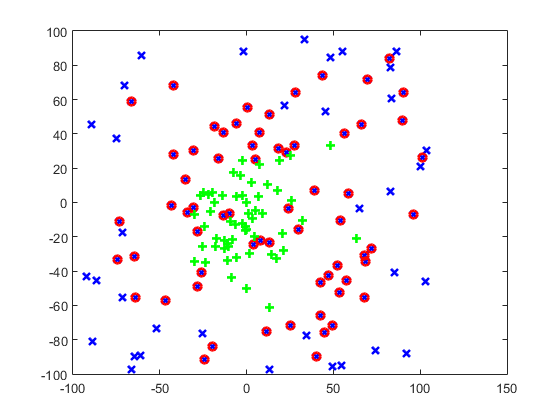
\includegraphics[width=10cm]{g2.png}   
		\caption{Exemplo de minimização da função $ x^2 + y^2 $}
		\label{fig:g2_x2y2}
	\end{center}
\end{figure}
\newpage



